% -----------------------------------------------------------------------------
% Matplotlib cheat sheet - Released under the BSD License
% -----------------------------------------------------------------------------
\documentclass[10pt,landscape,a4paper]{article}
\usepackage[utf8]{inputenc}
\usepackage[T1]{fontenc}

% --- Page layout -------------------------------------------------------------
\usepackage[right=2.5mm, left=2.5mm, top=2.5mm, bottom=2.5mm]{geometry}

% --- English stuff -----------------------------------------------------------
\usepackage[english]{babel}
\usepackage{xspace}
\usepackage{csquotes}

% --- Graphics ----------------------------------------------------------------
\usepackage{tikz}
\usepackage{graphicx}
\graphicspath{{./figures/}{./icons/}{./logos/}}
\usepackage[export]{adjustbox}

% --- Framed boxes ------------------------------------------------------------
\usepackage[framemethod=TikZ]{mdframed}
\mdfsetup{skipabove=0pt,skipbelow=0pt}
\usepackage{menukeys}

% --- URL, href and colors ----------------------------------------------------
\usepackage{xcolor}
\colorlet{citecolor}{black}
\colorlet{linkcolor}{black}
\colorlet{urlcolor}{black}
\usepackage[
  bookmarks=true,
  breaklinks=true,
  pdfborder={0 0 0},
  citecolor=citecolor,
  linkcolor=linkcolor,
  urlcolor=urlcolor,
  colorlinks=true,
  linktocpage=false,
  hyperindex=true,
  colorlinks=true,
  linktocpage=false,
  linkbordercolor=white]{hyperref}

% --- Tests -------------------------------------------------------------------
\usepackage{etoolbox}

% --- Fonts -------------------------------------------------------------------
\usepackage{fontspec}
\usepackage[babel=true]{microtype}
\defaultfontfeatures{Ligatures=TeX}
\setmainfont{Source Serif Pro}[
  Path = fonts/source-serif-pro/SourceSerifPro-, Extension = .otf,
  UprightFont= Light,
  ItalicFont = LightIt,
  BoldFont   = Regular,
  BoldItalicFont = It]
\setsansfont{Roboto}[
  Path = fonts/roboto/Roboto-, Extension = .ttf,
  UprightFont = Light,
  ItalicFont = LightItalic,
  BoldFont = Regular ]
\setmonofont{Source Code Pro}[
  Path = fonts/source-code-pro/SourceCodePro-, Extension = .otf,
  UprightFont = Light,
  BoldFont = Regular ]
\newfontfamily\RobotoCon{Roboto Condensed}[
  Path = fonts/roboto/RobotoCondensed-, Extension = .ttf,
  UprightFont = Regular,
  ItalicFont = Italic,
  BoldFont = Bold ]  
\newfontfamily\Roboto{Roboto}[
  Path = fonts/roboto/Roboto-, Extension = .ttf,
  UprightFont = Regular,
  ItalicFont = Italic,
  BoldFont = Black ]  

% --- Arrays ------------------------------------------------------------------
\usepackage{multicol}
\usepackage{colortbl}
\usepackage{array, multirow}

% --- Maths -------------------------------------------------------------------
\usepackage{amsmath}


% --- PDF comments ------------------------------------------------------------
\usepackage{pdfcomment}

% --- Default options ---------------------------------------------------------
\setlength\parindent{0pt}
\setlength{\tabcolsep}{2pt}
\baselineskip=0pt
\setlength\columnsep{0.5em}


% --- Macros ------------------------------------------------------------------
\newcommand{\button}[1]{\tikz[baseline=(X.base)]
  \node [fill=orange!40, rectangle, inner sep=2pt,rounded corners=1pt] (X) {#1};}

\newcommand{\API}[1]{\tikz[baseline=(X.base)]
  \node [fill=black!40, rectangle, inner sep=2pt,rounded corners=1pt] (X)
        {\href{#1}{\color{white}{\tiny \sffamily \textbf{API}}}};}

\newcommand{\READ}[1]{\tikz[baseline=(X.base)]
  \node [fill=black!40, rectangle, inner sep=2pt,rounded corners=1pt] (X)
        {\href{#1}{\color{white}{\tiny \sffamily \textbf{READ}}}};}

\newcommand{\api}[1]{\tikz[baseline=(X.base)]
  \node [fill=orange!40, rectangle, inner sep=2pt,rounded corners=1pt] (X)
        {\href{#1}{\color{white}{\tiny \sffamily \textbf{API}}}};}


\newcommand{\plot}[5]{%
  \begin{tabular}{@{}p{0.18\columnwidth}p{0.795\columnwidth}@{}}
    \adjustimage{width=0.18\columnwidth,valign=t}{#1} &
    {\ttfamily \scriptsize #2} \hfill \api{#3} \newline
    {\scriptsize #4}  \newline
    {\scriptsize #5 } \vspace{.7em}\\
  \end{tabular}}

\newcommand{\scale}[3]{%
  \begin{tabular}{@{}p{0.18\columnwidth}p{0.288\columnwidth}@{}}
    \adjustimage{width=0.18\columnwidth,valign=t}{#1} & {\ttfamily #2} \newline
    {\scriptsize #3}
  \end{tabular}}

\newcommand{\colormap}[1]{%
  \adjustimage{width=0.7\columnwidth,valign=c}{colormap-#1.pdf} &
  \tiny \ttfamily #1\\ \arrayrulecolor{white}\hline
}

\newcommand{\palette}[2]{%
  \adjustimage{width=0.7\columnwidth,valign=c}{colors-#1.pdf} &
  \tiny \ttfamily #2\\ \arrayrulecolor{white}\hline
}


\newcommand{\optional}[1]{\textcolor{gray}{#1}}
\newcommand{\mandatory}[1]{\textbf{#1}}
\newcommand{\parameter}[2]{%
  \expandafter\ifstrequal\expandafter{#1}{optional}%
                                     {\optional{#2}}{\mandatory{#2}}}
% --- Parameter: interpolation

\newcommand{\paramx}[1]{%
  \pdftooltip{\parameter{#1}{X}}
  {Horizontal coordinates of data point. 1D array like or scalar. }
}
  
\newcommand{\paramy}[1]{%
  \pdftooltip{\parameter{#1}{Y}}%
  {Vertical coordinates of data point. 1D array like or scalar. }
}

\newcommand{\paramfmt}[1]{%
  \pdftooltip{\parameter{#1}{fmt}}%
  {A format string, e.g. 'ro' for red circles. Format strings are just
   an abbreviation for quickly setting basic line properties. All of
   these and more can also be controlled by keyword arguments.}
}

\newcommand{\paramcolor}[1]{%
  \pdftooltip{\parameter{#1}{color}}%
  {Set line color.}
}

\newcommand{\parammarker}[1]{%
  \pdftooltip{\parameter{#1}{marker}}%
  {Set marker style.}
}

\newcommand{\paramlinestyle}[1]{%
  \pdftooltip{\parameter{#1}{linestyle}}%
  {Set line style.}
}

  
  \newcommand{\interpolation}[1]{%
  \pdftooltip{\parameter{#1}{interpolation}}
  {None, 'none', 'nearest', 'bilinear', 'bicubic', 'spline16', 'spline36',
   'hanning', 'hamming', 'hermite', 'kaiser', 'quadric', 'catrom', 'gaussian',
   'bessel', 'mitchell', 'sinc', 'lanczos'}
}

% --- Parameter: extent
\newcommand{\extent}{\pdftooltip{extent}{[left, right, bottom, top]}}

% --- Parameter: origin
\newcommand{\origin}{\pdftooltip{origin}{'upper', 'lower'}}

% --- Parameter: z
\newcommand{\Z}{\pdftooltip{z}{(M,N): an image with scalar data. The values are mappedto colors using normalization and a colormap.\textCR
(M, N, 3): an image with RGB values (0-1 float or 0-255 int)\textCR
(M, N, 4): an image with RGBA values (0-1 float or 0-255 int)}}

% --- Parameter: cmap
\newcommand{\cmap}{\pdftooltip{cmap}{
    Uniform: 'viridis', 'plasma', 'inferno', 'magma', 'cividis'\textCR
    \textCR
    Sequential: 'Greys', 'Purples', 'Blues', 'Greens', 'Oranges', 'Reds',
                'YlOrBr', 'YlOrRd', 'OrRd', 'PuRd', 'RdPu', 'BuPu',
                'GnBu', 'PuBu', 'YlGnBu', 'PuBuGn', 'BuGn', 'YlGn'\textCR
    \textCR
    Diverging: 'PiYG', 'PRGn', 'BrBG', 'PuOr', 'RdGy', 'RdBu',
               'RdYlBu', 'RdYlGn', 'Spectral', 'coolwarm', 'bwr',
               'seismic'\textCR
    \textCR
    Cyclic: 'twilight', 'twilight_shifted', 'hsv'\textCR
    \textCR
    Qualitative: 'Pastel1', 'Pastel2', 'Paired', 'Accent',
                 'Dark2', 'Set1', 'Set2', 'Set3', 'tab10',
                 'tab20', 'tab20b', 'tab20c'}}


\newenvironment{myboxed}[1]
{\begin{mdframed}[linecolor=black,
                  backgroundcolor=white,
                  outerlinewidth=0.25pt,
                  %roundcorner=0.25em,
                  innertopmargin=1ex,
                  topline=true,
                  rightline=true,
                  leftline=true,
                  bottomline=true,
                  linecolor=black!10,
                  frametitleaboveskip=0.5em,
                  frametitlebelowskip=0.5em,
                  innerbottommargin=.5\baselineskip,
                  innerrightmargin=.5em,
                  innerleftmargin=.5em,
                  %userdefinedwidth=1\textwidth,
                  frametitle={\scshape \bfseries \sffamily #1},
                  % frametitlerule=true,
                  %frametitlerulecolor=red,
                  frametitlebackgroundcolor=black!10,
                  frametitlerulewidth=2pt]}
{\end{mdframed}}





% -----------------------------------------------------------------------------
\begin{document}
\thispagestyle{empty}
% \footnotesize
\scriptsize

\begin{multicols*}{5}

  
\includegraphics[width=\columnwidth]{matplotlib.pdf}
  %\textbf{\Large \RobotoCon Matplotlib 3.2 cheat sheet}\\
  %{\ttfamily https://matplotlib.org} \hfill CC-BY 4.0
  % \bigskip
  \vspace{\fill}
  %\hspace{1mm} \small \url{https://matplotlib.org/}
  %\vspace{\fill}

  % --- Quick start -----------------------------------------------------------
  \begin{myboxed}{Quick start \hfill
      \API{https://matplotlib.org/tutorials/introductory/pyplot.html}}
  {\ttfamily \scriptsize
  import numpy as np\\
  import matplotlib as mpl\\
  import matplotlib.pyplot as plt\\
  \\
  \\
  X = np.linspace(0, 2*np.pi, 100)\\
  Y = np.cos(X)\\
  \\
  fig, ax = plt.subplots()\\
  ax.plot(X,Y,color='C1')\\
  \\
  plt.savefig(``figure.pdf'')\\
  plt.show() }
  \end{myboxed}
  \vspace{\fill}
    
  % --- Figure anatomy --------------------------------------------------------
  \begin{myboxed}{Anatomy of a figure}
  \includegraphics[width=\columnwidth]{anatomy.pdf}
  \end{myboxed}
  \vspace{\fill}
  % --- Layout ---------------------------------------------------------------
  \begin{myboxed}{Subplots layout \hfill
      \API{https://matplotlib.org/tutorials/intermediate/gridspec.html} }
  \plot{layout-subplot.pdf}{\textbf{subplot[s]}(cols,rows,…)}
       {https://matplotlib.org/api/_as_gen/matplotlib.pyplot.subplots.html}
       {\ttfamily fig, axs = plt.subplots(3,3)}
       {}
  \plot{layout-gridspec.pdf}{G = \textbf{gridspec}(cols,rows,…)}
       {https://matplotlib.org/api/_as_gen/matplotlib.gridspec.GridSpec.html}
       {\ttfamily ax = G[0,:]}{}
  \plot{layout-inset.pdf}{ax.\textbf{inset\_axes}(extent)}
       {https://matplotlib.org/api/_as_gen/matplotlib.axes.Axes.inset_axes.html}
       {}{}
  \plot{layout-divider.pdf}{d=\textbf{make\_axes\_locatable}(ax)}
       {https://matplotlib.org/mpl_toolkits/axes_grid/users/axes_divider.html}
       {\ttfamily ax=d.new\_horizontal('10\%')}{}
  \end{myboxed}
  \vspace{\fill}
  
  % --- Getting help ----------------------------------------------------------
  \begin{myboxed}{Getting help}
    
\includegraphics[height=.75em]{www.png}
    \href{https://matplotlib.org}
         {matplotlib.org}\\
    
\includegraphics[height=.75em]{github.png}
    \href{https://github.com/matplotlib/matplotlib/issues}
         {github.com/matplotlib/matplotlib/issues}\\
    
\includegraphics[height=.75em]{discourse.pdf}
    \href{https://discourse.matplotlib.org}
         {discourse.matplotlib.org}\\
    
\includegraphics[height=.75em]{stack-overflow.pdf}
    \href{https://stackoverflow.com/questions/tagged/matplotlib}
         {stackoverflow.com/matplotlib}\\
    
\includegraphics[height=.75em]{gitter.pdf}
    \href{https://gitter.im/matplotlib/matplotlib}
         {gitter.im/matplotlib}\\
    
\includegraphics[height=.75em]{twitter.pdf}
    \href{https://twitter.com/matplotlib}
         {twitter.com/matplotlib}\\
    
\includegraphics[height=.75em]{mail.pdf}
    \href{https://mail.python.org/mailman/listinfo/matplotlib-users}
         {Matplotlib users mailing list}
  \end{myboxed}

    
  % --- Basic plots -----------------------------------------------------------
  \begin{myboxed}{Basic plots}
  \plot{basic-plot.pdf}{\textbf{plot}([X],Y,[fmt],…)}
       {https://matplotlib.org/api/_as_gen/matplotlib.pyplot.plot.html}
       {\optional{X},
        \mandatory{Y},
        \optional{fmt},
        \optional{color},
        \optional{marker},
        \optional{linestyle}}
       {}
  \plot{basic-scatter.pdf}{\textbf{scatter}(X,Y,…)}
       {https://matplotlib.org/api/_as_gen/matplotlib.pyplot.scatter.html}
       {\mandatory{X},
        \mandatory{Y},
        \optional{[s]izes},
        \optional{[c]olors},
        \optional{markers},
        \optional{cmap}}
       {}
  \plot{basic-bar.pdf}{\textbf{bar[h]}(x,height,…)}
       {https://matplotlib.org/api/_as_gen/matplotlib.pyplot.bar.html}
       { \mandatory{x},
         \mandatory{height},
         \optional{width},
         \optional{bottom},
         \optional{align},
         \optional{color} }{}
  \plot{basic-imshow.pdf}{\textbf{imshow}(Z,[cmap],…)}
       {https://matplotlib.org/api/_as_gen/matplotlib.pyplot.imshow.html}
       { \mandatory{Z},
         \optional{cmap},
         \optional{interpolation},
         \optional{extent},
         \optional{origin} }
       {}
  \plot{basic-contour.pdf}{\textbf{contour[f]}([X],[Y],Z,,…)}
       {https://matplotlib.org/api/_as_gen/matplotlib.pyplot.contour.html}
       { \optional{X},
         \optional{Y},
         \mandatory{Z},
         \optional{levels},
         \optional{colors},
         \optional{extent},
         \optional{origin} }
       {}
  \plot{basic-quiver.pdf}{\textbf{quiver}([X],[Y],U,V,…)}
     {https://matplotlib.org/api/_as_gen/matplotlib.pyplot.quiver.html}
     { \optional{X},
       \optional{Y},
       \mandatory{U},
       \mandatory{V},
       \optional{C},
       \optional{units},
       \optional{angles} }
     {}
  \plot{basic-pie.pdf}{\textbf{pie}(X,[explode],…)}
       {https://matplotlib.org/api/_as_gen/matplotlib.pyplot.pie.html}
       {\mandatory{Z},
         \optional{explode},
         \optional{labels},
         \optional{colors},
         \optional{radius}}
       {}
   \plot{basic-text.pdf}{\textbf{text}(x,y,text,…)}
       {https://matplotlib.org/api/_as_gen/matplotlib.pyplot.text.html}
       {\mandatory{x},
        \mandatory{y},
        \mandatory{text},
        \optional{va},
        \optional{ha},
        \optional{size},
        \optional{weight},
        \optional{transform} }
       {}
   \plot{basic-fill.pdf}{\textbf{fill[\_between][x]}( … )}
       {https://matplotlib.org/api/_as_gen/matplotlib.pyplot.pie.html}
       {\mandatory{X},
        \optional{Y1},
        \optional{Y2},
        \optional{color},
        \optional{where} }
       {}
  \end{myboxed}
  \vspace{\fill}
  % --- Advanced plots --------------------------------------------------------
  \begin{myboxed}{Advanced plots}
  \plot{advanced-step.pdf}{\textbf{step}(X,Y,[fmt],…)}
     {https://matplotlib.org/api/_as_gen/matplotlib.pyplot.step.html}
     {\mandatory{X},
      \mandatory{Y},
      \optional{fmt},
      \optional{color},
      \optional{marker},
      \optional{where} }
     {}
  \plot{advanced-boxplot.pdf}{\textbf{boxplot}(X,…)}
     {https://matplotlib.org/api/_as_gen/matplotlib.pyplot.boxplot.html}
     { \mandatory{X},
       \optional{notch},
       \optional{sym},
       \optional{bootstrap},
       \optional{widths} }
     {}
  \plot{advanced-errorbar.pdf}{\textbf{errorbar}(X,Y,xerr,yerr,…)}
     {https://matplotlib.org/api/_as_gen/matplotlib.pyplot.errorbar.html}
     { \mandatory{X},
       \mandatory{Y},
       \optional{xerr},
       \optional{yerr},
       \optional{fmt} }
     {}
  \plot{advanced-hist.pdf}{\textbf{hist}(X, bins, …)}
     {https://matplotlib.org/api/_as_gen/matplotlib.pyplot.hist.html}
     {\mandatory{X},
      \optional{bins},
      \optional{range},
      \optional{density},
      \optional{weights}}
     {}
  \plot{advanced-violin.pdf}{\textbf{violinplot}(D,…)}
     {https://matplotlib.org/api/_as_gen/matplotlib.axes.Axes.violinplot.html}
     {\mandatory{D},
      \optional{positions},
      \optional{widths},
      \optional{vert} }
     {}
  \plot{advanced-barbs.pdf}{\textbf{barbs}([X],[Y], U, V, …)}
     {https://matplotlib.org/api/_as_gen/matplotlib.axes.Axes.violinplot.html}
     { \optional{X},
       \optional{Y},
       \mandatory{U},
       \mandatory{V},
       \optional{C},
       \optional{length},
       \optional{pivot},
       \optional{sizes} }
     {}
  \plot{advanced-event.pdf}{\textbf{eventplot}(positions,…)}
     {https://matplotlib.org/api/_as_gen/matplotlib.pyplot.eventplot.html}
     {\mandatory{positions},
       \optional{orientation},
       \optional{lineoffsets} }
     {}
  \plot{advanced-hexbin.pdf}{\textbf{hexbin}(X,Y,C,…)}
     {https://matplotlib.org/api/_as_gen/matplotlib.pyplot.hexbin.html}
     {\mandatory{X},
      \mandatory{Y},
      \optional{C},
      \optional{gridsize},
       \optional{bins} }
     {}
  \plot{advanced-xcorr.pdf}{\textbf{xcorr}(X,Y,…)}
     {https://matplotlib.org/api/_as_gen/matplotlib.pyplot.xcorr.html}
     {\mandatory{X},
      \mandatory{Y},
      \optional{normed},
      \optional{detrend} }
     {}
  \end{myboxed}


  % --- Scale ---------------------------------------------------------------
  \begin{myboxed}{Scales \hfill
    \API{https://matplotlib.org/api/scale_api.html}}
  {\ttfamily ax.\textbf{set\_[xy]scale}(scale,…)}
  \smallskip
  \scale{scale-linear.pdf}{\textbf{linear}}{any values}
  \scale{scale-log.pdf}{\textbf{log}}{values > 0}
  \scale{scale-symlog.pdf}{\textbf{symlog}}{any values}
  \scale{scale-logit.pdf}{\textbf{logit}}{0 < values <  1}
  \end{myboxed}
  %
  \vspace{\fill}
  %
  % --- Projections -----------------------------------------------------------
  \begin{myboxed}{Projections \hfill
      \API{https://matplotlib.org/api/projections_api.html}}
  {\ttfamily \textbf{subplot}(…,projection=p)}
  \smallskip
  \scale{projection-polar.pdf}{p='polar'}{}
  \scale{projection-3d.pdf}{p='3d'}{}
%       {https://matplotlib.org/api/projections_api.html}
%       {}
%       {}
  %% \plot{projection-3d.pdf}{p='3d'}
  %%      {https://matplotlib.org/api/toolkits/mplot3d.html}
  %%      {}
  %%      {}
  \plot{projection-cartopy.pdf}{p=Orthographic()}
       {https://matplotlib.org/api/toolkits/mplot3d.html}
       {from cartopy.crs import Cartographic}
       {}
  \end{myboxed}
  %
  \vspace{\fill}
  %
  % --- Linestyles ---------------------------------------------------------------
  \begin{myboxed}{Lines \hfill
      \API{https://matplotlib.org/gallery/lines_bars_and_markers/linestyles.html}}
  \includegraphics[width=\columnwidth]{linestyles.pdf}
  \end{myboxed}
  %
  \vspace{\fill}
  %
  % --- Markers ---------------------------------------------------------------
  \begin{myboxed}{Markers \hfill
                \API{https://matplotlib.org/api/markers_api.html}}
      \includegraphics[width=\columnwidth]{markers.pdf}
  \end{myboxed}
  %
  \vspace{\fill}
  %
  % --- Colors ---------------------------------------------------------------
  \begin{myboxed}{Colors \hfill
      \API{https://matplotlib.org/tutorials/colors/colors.html}}
    %  mpl.colors.to\_rbga(\textbf{color})\smallskip\\
    \def\arraystretch{0.5}
    \begin{tabular}{@{}p{0.7\columnwidth}p{0.25\columnwidth}@{}}
      \palette{cycle}{'Cn'}
      \palette{raw}{ 'x' }
      \palette{name}{'name'}
      \palette{rgba}{(R,G,B[,A])}
      \palette{HexRGBA}{'\#RRGGBB[AA]'}
      \palette{grey}{'x.y'}
    \end{tabular}
  \end{myboxed}
  %
  \vspace{\fill}
  %
  

  % --- Colormaps -------------------------------------------------------------
  \begin{myboxed}{Colormaps \hfill
      \API{https://matplotlib.org/tutorials/colors/colormaps.html}}
    {\ttfamily plt.\textbf{get\_cmap}(name) \smallskip\\}
    \def\arraystretch{0.5}
    \begin{tabular}{@{}p{0.7\columnwidth}p{0.25\columnwidth}@{}}
      \scriptsize \rule{0pt}{1.25em}Uniform & \\
      \colormap{viridis} \colormap{magma} \colormap{plasma}
      %
      \scriptsize \rule{0pt}{1.25em}Sequential &\\
      \colormap{Greys} \colormap{YlOrBr} \colormap{Wistia}
      %
      \scriptsize \rule{0pt}{1.25em}Diverging &\\
      \colormap{Spectral} \colormap{coolwarm} \colormap{RdGy}
      %
      \scriptsize \rule{0pt}{1.25em}Qualitative &\\
      \colormap{tab10} \colormap{tab20}
      %
      \scriptsize \rule{0pt}{1.25em}Cyclic &\\
      \colormap{twilight} % \colormap{hsv}
    \end{tabular}
  \end{myboxed}

  % --- Ticks locators --------------------------------------------------------
  \begin{myboxed}{Tick locators \hfill
    \API{https://matplotlib.org/api/ticker_api.html}}
    {\tiny \ttfamily
      from matplotlib import ticker\\
      ax.[xy]axis.set\_[minor|major]\_locator(\textbf{locator})\par
      \vspace{1em}
      \hspace{-1em}\includegraphics[width=\columnwidth]{tick-locators.pdf}
      }
  \end{myboxed}
  %
  \vspace{\fill}
  %
  \begin{myboxed}{Tick formatters \hfill
    \API{https://matplotlib.org/api/ticker_api.html}}
    {\tiny \ttfamily
      from matplotlib import ticker\\
      ax.[xy]axis.set\_[minor|major]\_formatter(\textbf{formatter})\par
      \vspace{1em}
      \hspace{-1em}\includegraphics[width=\columnwidth]{tick-formatters.pdf}
    }
  \end{myboxed}
  %
  \vspace{\fill}
  %
  \begin{myboxed}{Ornaments}
    {\ttfamily ax.\textbf{legend}(…) \hfill
    \api{https://matplotlib.org/api/_as_gen/matplotlib.pyplot.legend.html}}\\
     handles, labels, loc, title, frameon\smallskip\\
    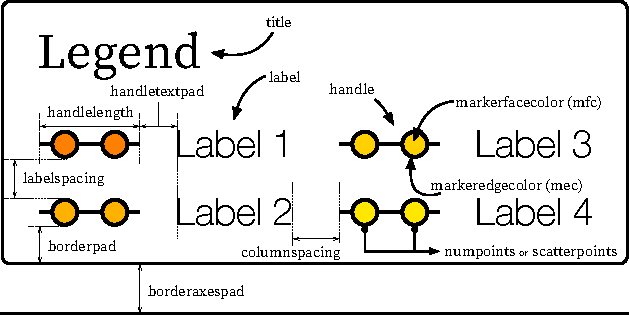
\includegraphics[width=0.9\columnwidth]{legend.pdf}
    \medskip\\
    %
    {\ttfamily ax.\textbf{colorbar}(…)} \hfill
    \api{https://matplotlib.org/api/_as_gen/matplotlib.pyplot.colorbar.html}\\
    mappable, ax, cax, orientation \smallskip\\
    \includegraphics[width=\columnwidth]{colorbar.pdf}\\
    \medskip\\
    %
    {\ttfamily ax.\textbf{annotate}(…)} \hfill
    \api{https://matplotlib.org/api/_as_gen/matplotlib.pyplot.annotate.html}\\
    \mandatory{text},
    \mandatory{xy},
    \mandatory{xytext},
    \optional{xycoords},
    \optional{textcoords},
    \optional{arrowprops}
    \smallskip\\
    \includegraphics[width=\columnwidth]{annotate.pdf}\\
    %
  \end{myboxed}
  %
  \vspace{\fill}
  %
  \begin{myboxed}{Event handling \hfill
      \API{https://matplotlib.org/users/event_handling.html}}
    {\ttfamily \scriptsize
      fig, ax = plt.subplots()\par
      \par
      def on\_click(event):\par
      ~~print(event)\par
      fig.canvas.mpl\_connect(\par
      ~~'button\_press\_event', on\_click)\par
    }
  \end{myboxed}

  %
  % \vspace{\fill}
  %
  \begin{myboxed}{Animation \hfill
      \API{https://matplotlib.org/api/animation_api.html}}
  {\ttfamily \scriptsize
  import matplotlib.animation as mpla\par
  ~\par
  T = np.linspace(0,2*np.pi,100)\par
  S = np.sin(T)\par
  line, = plt.plot(T, S)\par
  def animate(i):\par
  ~~line.set\_ydata(np.sin(T+i/50))\par
  anim = mpla.FuncAnimation(\par
  ~~plt.gcf(), animate, interval=5)\par
  plt.show()\par
  }
  \end{myboxed}
  %
  \vspace{\fill}
  %
  \begin{myboxed}{Styles \hfill
      \API{https://matplotlib.org/tutorials/introductory/customizing.html}}
    \setlength{\fboxsep}{0pt}%
    \setlength{\fboxrule}{.25pt}%
              {\ttfamily plt.style.use(\textbf{style})\medskip}\\
    \fbox{\includegraphics[width=.32\columnwidth]{style-default.pdf}}
    \fbox{\includegraphics[width=.32\columnwidth]{style-classic.pdf}}
    \fbox{\includegraphics[width=.32\columnwidth]{style-grayscale.pdf}}
    \fbox{\includegraphics[width=.32\columnwidth]{style-ggplot.pdf}}
    \fbox{\includegraphics[width=.32\columnwidth]{style-seaborn.pdf}}
    \fbox{\includegraphics[width=.32\columnwidth]{style-fast.pdf}}
    \fbox{\includegraphics[width=.32\columnwidth]{style-bmh.pdf}}
    \fbox{\includegraphics[width=.32\columnwidth]{style-Solarize_Light2.pdf}}
    \fbox{\includegraphics[width=.32\columnwidth]{style-seaborn-notebook.pdf}}
    %% \fbox{\includegraphics[width=.24\columnwidth]{style-default.pdf}}
    %% \fbox{\includegraphics[width=.24\columnwidth]{style-classic.pdf}}
    %% \fbox{\includegraphics[width=.24\columnwidth]{style-grayscale.pdf}}
    %% \fbox{\includegraphics[width=.24\columnwidth]{style-ggplot.pdf}}
    %% \fbox{\includegraphics[width=.24\columnwidth]{style-seaborn.pdf}}
    %% \fbox{\includegraphics[width=.24\columnwidth]{style-fast.pdf}}
    %% \fbox{\includegraphics[width=.24\columnwidth]{style-bmh.pdf}}
    %% \fbox{\includegraphics[width=.24\columnwidth]{style-Solarize_Light2.pdf}}
  \end{myboxed}
  %
  \vspace{\fill}
  %
  \begin{myboxed}{Quick reminder}
  {\ttfamily
    ax.\textbf{grid}()\\
    ax.patch.\textbf{set\_alpha}(0)\\
    ax.\textbf{set\_[xy]lim}(vmin, vmax)\\
    ax.\textbf{set\_[xy]label}(label)\\
    ax.\textbf{set\_[xy]ticks}(list)\\
    ax.\textbf{set\_[xy]ticklabels}(list)\\
    ax.\textbf{set\_[sup]title}(title)\\
    ax.\textbf{tick\_params}(width=10, …)\\
    ax.\textbf{set\_axis\_[on|off]}()\\
    \\
    plt.\textbf{tight\_layout}()\\
    plt.\textbf{gcf}(), plt.\textbf{gca}()\\
    mpl.\textbf{rc}('axes', linewidth=1, …)\\
    fig.patch.\textbf{set\_alpha}(0)\\
    \verb|text=r'$\frac{-e^{i\pi}}{2^n}$'|}
  \end{myboxed}
  %
  \vspace{\fill}
  %
  %% % --- Toolkits --------------------------------------------------------------
  %% \begin{myboxed}{Toolkits and libraries}
  %%   \href{https://matplotlib.org/basemap/}{Basemap} ---
  %% \href{https://scitools.org.uk/cartopy/docs/latest/}{Cartopy} ---
  %% \href{https://geopandas.org/}{GeoPandas} ---
  %% \href{https://residentmario.github.io/geoplot/index.html}{Geoplot} ---
  %% \href{https://github.com/yhat/ggpy}{GGPlot} ---
  %% \href{http://holoviews.org/}{Holoviews} ---
  %% \href{https://seaborn.pydata.org/}{Seaborn} ---
  %% \href{https://gr-framework.org/}{GR Framework} ---
  %% \href{https://www.scikit-yb.org/en/latest/}{Yellowbrick}
  %% \end{myboxed}
  %% %
  %% \vspace{\fill}
  %
  \begin{myboxed}{Keyboard shortcuts \hfill
    \API{https://matplotlib.org/users/navigation_toolbar.html}}
    \def\arraystretch{1.25}
    \begin{tabular}{ll}
      \keys{\ctrl+s} Save        & \keys{\ctrl+w} Close plot\\
      \keys{r} Reset view        & \keys{f} Fullscreen 0/1\\
      \keys{f} View forward      & \keys{b} View back\\
      \keys{p} Pan view          & \keys{o} Zoom to rect\\
      \keys{x} X pan/zoom        & \keys{y} Y pan/zoom\\
      \keys{g} Minor grid 0/1    & \keys{G} Major grid 0/1\\
      \keys{l} X axis log/linear & \keys{L} Y axis log/linear\\
      %\keys{l} & Toggle y linear / log axis\\
    \end{tabular}
  \end{myboxed}
  %
  \vspace{\fill}
  %
  \begin{myboxed}{Ten Simple Rules \hfill
      \READ{https://journals.plos.org/ploscompbiol/article?id=10.1371/journal.pcbi.1003833}}
    1. Know Your Audience\\
    2. Identify Your Message\\
    3. Adapt the Figure\\
    4. Captions Are Not Optional\\
    5. Do Not Trust the Defaults\\
    6. Use Color Effectively\\
    7. Do Not Mislead the Reader\\
    8. Avoid “Chartjunk”\\
    9. Message Trumps Beauty\\
    10. Get the Right Tool
  \end{myboxed} 
\end{multicols*}

\begin{multicols*}{5}
  \begin{myboxed}{Axes adjustements\hfill
      \API{https://matplotlib.org/api/_as_gen/matplotlib.pyplot.subplots_adjust.html}}
    plt.\textbf{subplot\_adjust}( … )\\

    \includegraphics[width=\columnwidth]{adjustments.pdf}
  \end{myboxed}
  %
  \vspace{\fill}
  %
  \begin{myboxed}{Extent \& origin \hfill
      \API{https://matplotlib.org/tutorials/intermediate/imshow_extent.html} }
    plt.\textbf{imshow}( extent=…, origin=… )\\

    \includegraphics[width=\columnwidth]{extents.pdf}
  \end{myboxed}
  %
  \vspace{\fill}
  %
  \begin{myboxed}{Text alignments \hfill
      \API{https://matplotlib.org/tutorials/text/text_props.html} }
    plt.\textbf{text}( …, ha=… , va=…, … )\\

    \includegraphics[width=\columnwidth]{text-alignments.pdf}
  \end{myboxed}
  %
  \vspace{\fill}
  %
  \begin{myboxed}{Text parameters  \hfill
      \API{https://matplotlib.org/tutorials/text/text_props.html}}
    plt.\textbf{text}( …, family=… , size=…, weight = …)\\
    plt.\textbf{text}( …, fontproperties = … )\\

    \includegraphics[width=\columnwidth]{fonts.pdf}
  \end{myboxed}


  \begin{myboxed}{Uniform colormaps}
    \begin{tabular}{@{}p{0.7\columnwidth}p{0.25\columnwidth}@{}}
      \scriptsize \rule{0pt}{1.25em}\noindent
      \colormap{viridis}
      \colormap{plasma}
      \colormap{inferno}
      \colormap{magma}
      \colormap{cividis}
    \end{tabular}
  \end{myboxed}
  %
  \vspace{\fill}
  %
  \begin{myboxed}{Sequential colormaps}
    \begin{tabular}{@{}p{0.7\columnwidth}p{0.25\columnwidth}@{}}
      \scriptsize \rule{0pt}{1.25em}\noindent
      \colormap{Greys}
      \colormap{Purples}
      \colormap{Blues}
      \colormap{Greens}
      \colormap{Oranges}
      \colormap{Reds}
      \colormap{YlOrBr}
      \colormap{YlOrRd}
      \colormap{OrRd}
      \colormap{PuRd}
      \colormap{RdPu}
      \colormap{BuPu}
      \colormap{GnBu}
      \colormap{PuBu}
      \colormap{YlGnBu}
      \colormap{PuBuGn}
      \colormap{BuGn}
      \colormap{YlGn}
    \end{tabular}
  \end{myboxed}
  %
  \vspace{\fill}
  %
  \begin{myboxed}{Diverging colormaps}
    \begin{tabular}{@{}p{0.7\columnwidth}p{0.25\columnwidth}@{}}
      \scriptsize \rule{0pt}{1.25em}\noindent
      \colormap{PiYG}
      \colormap{PRGn}
      \colormap{BrBG}
      \colormap{PuOr}
      \colormap{RdGy}
      \colormap{RdBu}
      \colormap{RdYlBu}
      \colormap{RdYlGn}
      \colormap{Spectral}
      \colormap{coolwarm}
      \colormap{bwr}
      \colormap{seismic}
    \end{tabular}
  \end{myboxed}
  %
  \vspace{\fill}
  %
  \begin{myboxed}{Qualitative colormaps}
    \begin{tabular}{@{}p{0.7\columnwidth}p{0.25\columnwidth}@{}}
      \scriptsize \rule{0pt}{1.25em}\noindent
      \colormap{Pastel1}
      \colormap{Pastel2}
      \colormap{Paired}
      \colormap{Accent}
      \colormap{Dark2}
      \colormap{Set1}
      \colormap{Set2}
      \colormap{Set3}
      \colormap{tab10}
      \colormap{tab20}
      \colormap{tab20b}
      \colormap{tab20c}
    \end{tabular}
  \end{myboxed}
  %
  \vspace{\fill}
  %
  \begin{myboxed}{Miscellaneous colormaps}
    \begin{tabular}{@{}p{0.7\columnwidth}p{0.25\columnwidth}@{}}
      \scriptsize \rule{0pt}{1.25em}\noindent
      \colormap{terrain}
      \colormap{ocean}
      \colormap{cubehelix}
      \colormap{rainbow}
      \colormap{twilight}
    \end{tabular}
  \end{myboxed}

  
  
  \begin{myboxed}{Color names \hfill
      \API{https://matplotlib.org/api/colors_api.html} }
    \includegraphics[width=\columnwidth]{colornames.pdf}
  \end{myboxed}
  %
  \vspace{\fill}
  %
  \begin{myboxed}{Image interpolation
      \hfill \API{https://matplotlib.org/gallery/images_contours_and_fields/interpolation_methods.html} }
        \smallskip
%%    plt.\textbf{imshow}(…, interpolation=…)\\
%%    plt.\textbf{contour[f]}(…, interpolation=…)\\
    \includegraphics[width=\columnwidth]{interpolations.pdf}
  \end{myboxed}

  
  \begin{myboxed}{Legend placement}
    \includegraphics[width=\columnwidth]{legend-placement.pdf}
    plt.\textbf{legend}(loc="string", bbox\_to\_anchor=(x,y))\\
    \begin{tabular}{@{}p{0.33\columnwidth}
                       p{0.33\columnwidth}
                       p{0.33\columnwidth}@{}}
      \scriptsize \rule{0pt}{1.25em}\noindent
      1: lower left & 2: lower center & 3: lower right\\
      4: left       & 5: center       & 6: right\\
      7: upper left & 8: upper center & 9: upper right\\
    \end{tabular}

    \begin{tabular}{@{}p{0.495\columnwidth}
                       p{0.495\columnwidth}@{}}
      \scriptsize \rule{0pt}{1.25em}\noindent
      A: upper right / (-.1,.9) & B: right / (-.1,.5)\\
      C: lower right / (-.1,.1) & D: upper left / (-.1,-.1)\\
      E: upper center / (.5,-.1) & F: upper right / (.9,-.1)\\
      G: lower left / (1.1,.1) & H: left / (1.1,.5)\\
      I: upper left / (1.1,.9) & J: lower right / (.9,1.1)\\
      K: lower center / (.5,1.1) & L: lower left / (.1,1.1)
    \end{tabular}  
  \end{myboxed}

  \vfill\null \columnbreak
  
  %
  \begin{myboxed}{How do I …}
    \textbf{… resize a figure?}\\
    \hspace*{2.5mm}~$\rightarrow$ fig.set\_size\_inches(w,h)\\
    \textbf{… save a figure?}\\
    \hspace*{2.5mm}~$\rightarrow$ plt.savefig("figure.pdf")\\
    \textbf{… save a transparent figure?}\\
    \hspace*{2.5mm}~$\rightarrow$ plt.savefig("figure.pdf", transparent=True)\\
    \textbf{… clear a figure?}\\
    \hspace*{2.5mm}~$\rightarrow$ ax.clear()\\
    \textbf{… close all figures?}\\
    \hspace*{2.5mm}~$\rightarrow$ plt.close("all")\\
    \textbf{… remove ticks?}\\
    \hspace*{2.5mm}~$\rightarrow$ ax.set\_xticks([])\\
    \textbf{… remove tick labels ?}\\
    \hspace*{2.5mm}~$\rightarrow$ ax.set\_[xy]ticklabels([])\\
    \textbf{… rotate tick labels ?}\\
    \hspace*{2.5mm}~$\rightarrow$ plt.[xy]ticks(rotation=90)\\
    \textbf{… hide top spine?}\\
    \hspace*{2.5mm}~$\rightarrow$ ax.spines['top'].set\_visible(False)\\
    \textbf{… hide legend border?}\\
    \hspace*{2.5mm}~$\rightarrow$  plt.legend(frameon=False)\\
    \textbf{… show error as shaded region?}\\
    \hspace*{2.5mm}~$\rightarrow$ ax.fill\_between(X, Y+error, Y-error)\\
    \textbf{… draw a rectangle?}\\
    \hspace*{2.5mm}~$\rightarrow$  ax.add\_patch(plt.Rectangle((0, 0),1,1)\\
    \textbf{… draw a vertical line?}\\
    \hspace*{2.5mm}~$\rightarrow$  ax.axvline(x=0.5)\\
    \textbf{… draw outside frame?}\\
    \hspace*{2.5mm}~$\rightarrow$  ax.plot(…, clip\_on=False)\\
    \textbf{… use transparency?}\\
    \hspace*{2.5mm}~$\rightarrow$  ax.plot(…, alpha=0.25)\\
    \textbf{… convert an RGB image into a gray image? }\\
    \hspace*{2.5mm}~$\rightarrow$  gray = 0.2989*R+0.5870*G+0.1140*B\\
    \textbf{… set figure background color?}\\
    \hspace*{2.5mm}~$\rightarrow$ fig.patch.set\_facecolor(``grey'')\\
    \textbf{… get a reversed colormap?}\\
    \hspace*{2.5mm}~$\rightarrow$ plt.get\_cmap(``viridis\_r'')\\
    \textbf{… get a discrete colormap?}\\
    \hspace*{2.5mm}~$\rightarrow$ plt.get\_cmap(``viridis'', 10)\\
    \textbf{… show a figure for one second?}\\
    \hspace*{2.5mm}~$\rightarrow$ plt.show(block=False), time.sleep(1)
  \end{myboxed}
  %
  \vspace{\fill}
  %
  \begin{myboxed}{Performance tips}
    \smallskip
    {\ttfamily \fontsize{6pt}{7pt}\selectfont
    \textcolor{red}{scatter(X, Y)  \hfill slow}\\
    plot(X, Y, marker="o", ls="")  \hfill fast\\
    \hrule \smallskip
    \textcolor{red}{for i in range(n): plot(X[i]) \hfill slow}\\
    plot(sum([x+[None] for x in X],[])) \hfill fast\\
    \hrule \smallskip
    \textcolor{red}{cla(), imshow(…), canvas.draw() \hfill slow}\\
    im.set\_data(…), canvas.draw() \hfill fast\smallskip
    }
  \end{myboxed}
  %
  \vspace{\fill}
  %
  \begin{myboxed}{Beyond Matplotlib}
        \smallskip
    \href{https://seaborn.pydata.org/}{\textbf{Seaborn}}: Statistical Data Visualization\\
    \href{https://scitools.org.uk/cartopy/docs/latest/}{\textbf{Cartopy}}: Geospatial Data Processing\\
    \href{https://yt-project.org/doc/index.html}{\textbf{yt}}: Volumetric data Visualization\\
    \href{https://mpld3.github.io}{\textbf{mpld3}}: Bringing Matplotlib to the browser\\
    \href{https://datashader.org/}{\textbf{Datashader}}: Large data processing pipeline\\
    \href{https://plotnine.readthedocs.io/en/latest/}{\textbf{plotnine}}: A Grammar of Graphics for Python
  \end{myboxed}
  %
  \begin{center}
  \href{https://github.com/matplotlib/cheatsheets}{Matplotlib Cheatsheets} (c) 2020 Nicolas P. Rougier\\
  Released under a CC-BY 4.0 International License\\
  \smallskip
  
\includegraphics[width=\columnwidth]{numfocus.png}
  \end{center}
  
\end{multicols*}
\end{document}

